\chapter{State of the Art} \label{chap:sota}

\section*{}

This chapter starts with an overview of online marketing in the last few years, followed by a review of the data mining algorithms that can be used to solve the same kind of problems as this thesis.

\section{Online Advertising Overview}\label{sec:adover}

Before entering in details about the state of the art of the technologies that can be used to
solve the presented problem, it is better to explain some basic concepts about the world of online advertising.

All advertising has the main purpose of getting a message to the people that will impact or influence them in some way,
therefore the same goal is applied to online advertising.
One of the metrics of advertising are impressions, which correspond to the number of times a user sees the message (the ad).\cite{kOA}
\textbf{Ads} can present itself in various sizes\cite{kOA2}, forms and locations \cite{kOA3}, and these characteristics are chosen both by the advertiser
and the publisher to better serve their purpose.
\textbf{Campaigns} are composed by two big parts, which are the ads that compose it and the target population that they pretend to reach,
including the rules of this targeting. For example, \textbf{frequency capping} to limit the number of times the same advertising is shown to the user \cite{kOA},
avoiding, in this way, showing the same ad multiple times in a row to the same user, that can lead to a bad response from his part.\cite{Buchbinder20141}

Nowadays, the main pricing models of online advertising are:
\begin{itemize}
\item\textbf{Cost-per-Mile (CPM)} where the advertiser pays per impression. The main
problem of this model is the advertiser must pay to the publisher even
if the ad doesn't lead to any profit.
\item\textbf{Cost-per-Click (CPC)} where the advertiser pays per click to the publisher. This model is more expensive per unit\cite{Performics}, but on overall can be more
profitable\cite{Performics} if the audience of the websites where the ad is imprinted is more interested in that kind of product/service\cite{Andrea2004}.
\item\textbf{Cost-per-lead (CPL)} where the advertiser pays for a lead. If this model is being used the advertiser doesn't pay per number of impressions nor per clicks. Instead, pays only
if he gets valid information about the user, like the information of a sign up form for a community.
\item\textbf{Cost-per-Action (CPA)} or \textbf{Cost-per-Order (CPO)} where the advertiser is charged per buy or action. This model is similar to CPL but has in mind an instantaneous return of
the investment.
\end{itemize}

Traditionally, publishers sell their space to advertisers in bulk (\textbf{Ad networks}) this method has its \textit{ups} and \textit{downs}.
The obvious \textit{up} is that sometimes the advertiser gets premium spots at low prices.
On the other hand, one of the biggest drawbacks is that when the advertiser buys the impressions as a
closed package, sometimes impressions are not maximized in terms of profit.
Other problem of traditional methods that, although the \emph{CPA} and \emph{CPL} pricing methods minimize the risk for the advertiser, the responsibility of
optimizing conversion rate\footnote{ See, e.g., \url{http://www.marketingterms.com/dictionary/conversion_rate/}} is still
on the ad network hands.\cite{Yuan:2013:RBO:2501040.2501980}

In the past few years, a new model called \textbf{Real Time Bidding (RTB)}\index{Real Time Bidding}\index{RTB} has been gaining terrain \cite{Adfonic}.
\emph{RTB} is a market where publishers offer his advertisement space and advertisers bid over it in real time. This allow publishers to get
the best value for their space and advertisers get the best placement for their advertisement.

There are three main players in the world of \emph{RTB}\index{Real Time Bidding}:
\begin{itemize}
\item\label{itm:dsp} The \textbf{Demand Side Platform (DSP)}\index{DSP} is a tool used by the advertisers to act on their behalf on the \emph{RTB}. \emph{DSPs}\index{DSP} allows them to set
their campaigns' parameters and to monitor the performance of the campaign. This way the advertisers try to get the best performance of their campaigns because 
\emph{DSPs} use algorithms driven by performance data.\cite{Gern201230}
\item\label{itm:ssp} The \textbf{Publisher} provides the inventory, that is comprised by accesses made by users. In some cases, the publisher uses \textbf{Supply Side Platforms}.
\emph{SSPs} help the publisher to better manage his inventory, and even let him set a reserve price for their inventory.\cite{Yuan:2013:RBO:2501040.2501980}
\item\label{itm:adex} The \textbf{Ad Exchange} looks a little like a stock exchange, but in reality is a software platform that mediates the exchange. This exchange takes place in
a few milliseconds while the page loads.
\end{itemize}

\emph{RTB} allows some features of paid search advertising everywhere \cite{Gern201230}, because it allows the advertiser to better select
the inventory\footnote{ this inventory is made of user accesses} where he wants their campaigns to run on.
The flexibility that \emph{RTB} gives to all the intervinients of this exchange is what demands the necessity of predicting the future inventory, to
better access its value.



\section{Data Mining}\label{sec:datamining}
%\begin{quote}
''Data mining is about solving problems by analyzing data already present in databases.''\cite[p. 5]{Witten:2005:DMP:1205860}
%\end{quote}
. Furthermore, consists in a vast number of techniques used to find interesting patterns in large datasets and translate
that huge quantity of raw data in information and/or knowledge. 

Data mining uses techniques from various fields, mostly from mathematics and computer science,
such as artificial intelligence, machine learning and statistics.
Data mining is sometimes referred as the natural evolution of information technologies \cite[p. 1]{HanKam06}

There are lots of methods of data mining, which can be separated in two groups: descriptive data mining and predictive
data mining \cite{Fayyad96knowledgediscovery}.
The main focus of the first group is to find the underlying structure of a given dataset, which methods try to find relationships and connections
between the values, without have the goal of predicting the future. On the other hand,
predictive data mining goal is to predict explicit values from patterns found on the original data set. These methods are used to build models based on past
events that can be used to predict future events.
This division is not always sharp and in some cases an algorithm mixes the two methods (predictive \& descriptive)\cite{Fayyad96knowledgediscovery}.

According to previous statements it is easy to notice that data mining doesn't apply only to one set of problems and can be used to solve many different types of
problems. The most common family of problem types are:
\begin{itemize}
\item \textbf{Anomaly Detection} tries to discover abnormal data on the dataset. This can be useful for identifying suspicious activity on a bank
account log for example.
\item \textbf{Classification} aims to identify which of a given set of
categories a new observation belongs to.
\item \textbf{Clustering} aims to grouping similar data together, in a finite number of categories, without prior knowledge of
the characteristics of each group or the data.
\item \textbf{Dependency modeling} tries to find associations between variables. For example, trying to find out which clothes go well together.
\item \textbf{Summarization} provides an overview of the dataset, sometimes including visual representation and/or report generation.
\item \textbf{Regression} tries to predict the value of a quantitative variable
given a new observation.
\end{itemize}

\subsection{Classification Algorithms}\label{sec:classification}

\subsubsection{Decision Trees}

Decision trees algorithms use a decision tree as a predictive model where all internal nodes (non-leaf nodes) are a test for the value of an attribute that will
ultimately lead to a leaf node with the class attribute value (see example in figure~\ref{fig:dtree}).
In other words, the selection of the class value is only based on the attribute values of the entry.\cite{HanKam06}

\begin{figure}[h]
  \begin{center}
    \leavevmode
    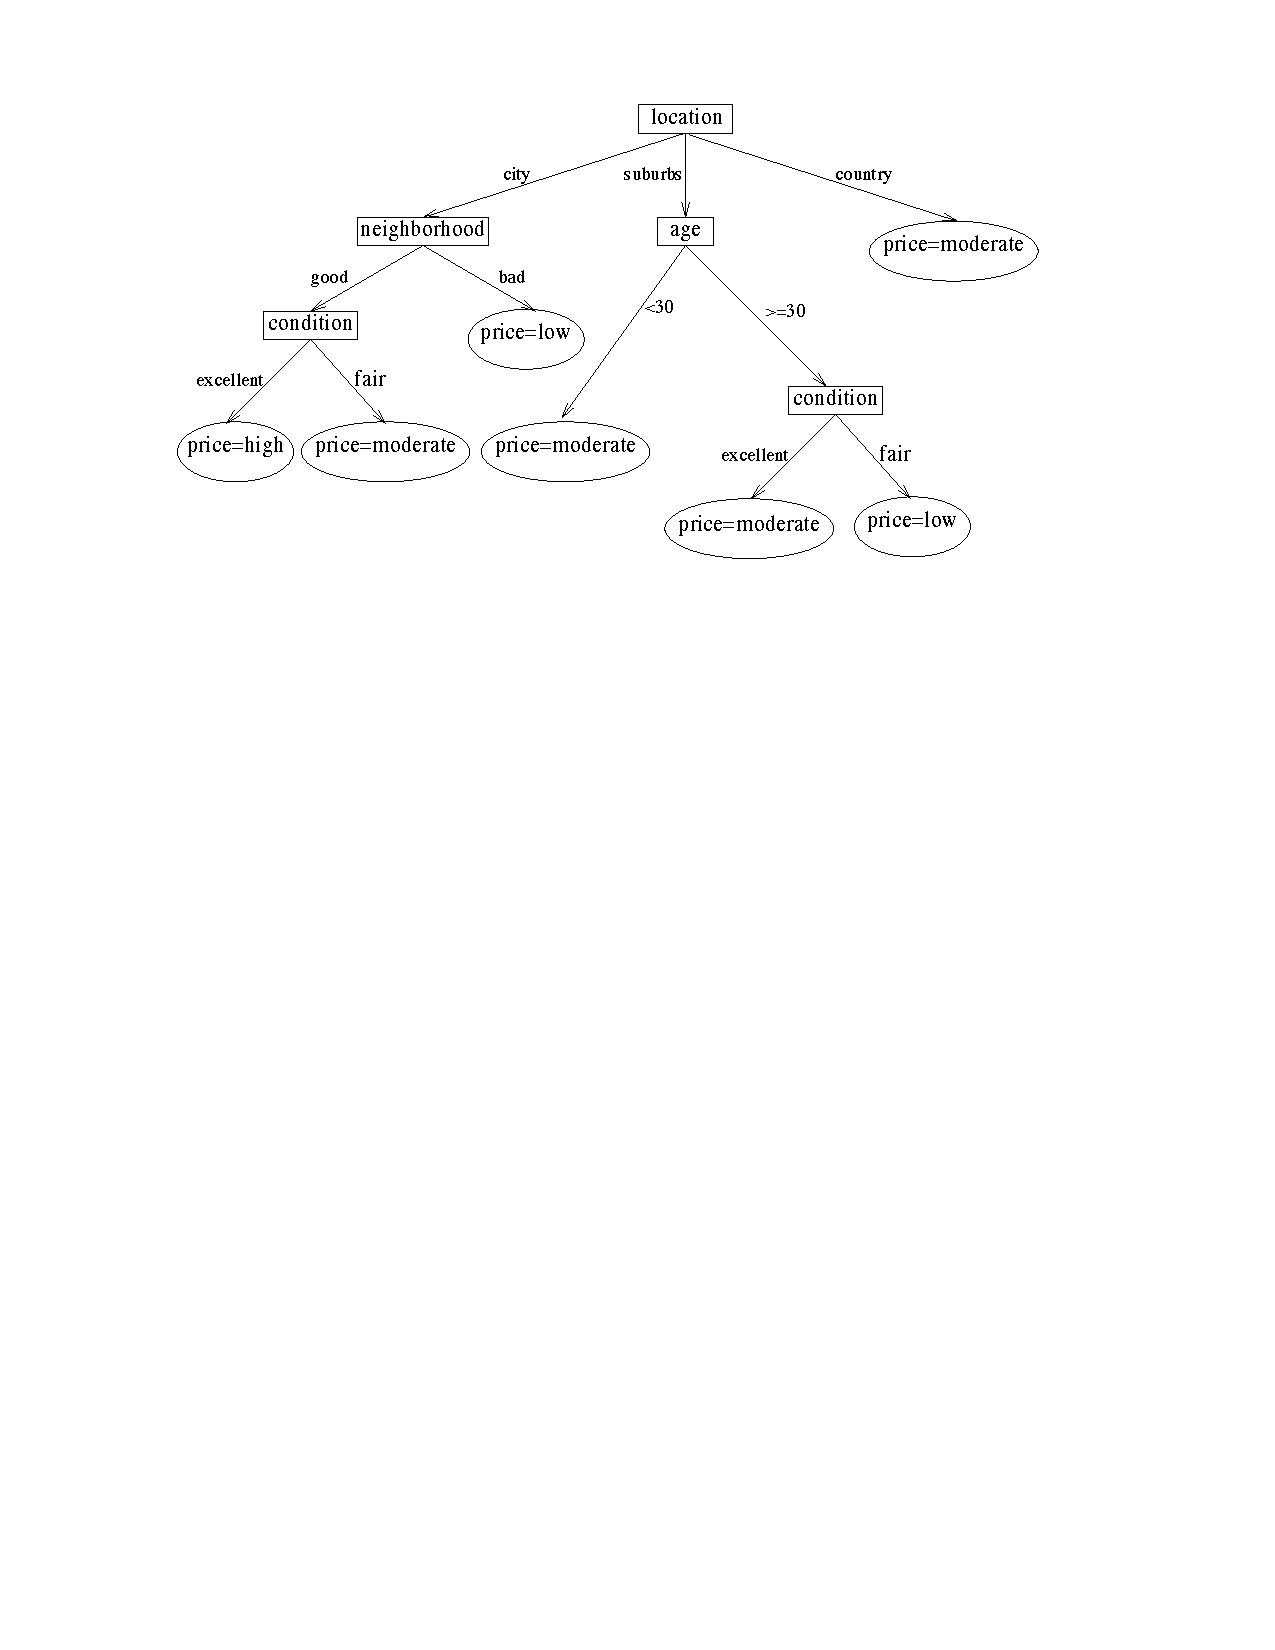
\includegraphics[width=0.86\textwidth]{dt}
    \caption{Example of a decision tree, Rectangles represent internal nodes and ovals represent leaf nodes (possible solution)\cite{KER:70953}}
    \label{fig:dtree}
  \end{center}
\end{figure}

Decision tree classifiers can be used in large datasets with high dimensional data and still be fast and easy to understand its result.
One of its' main advantages due to its white box model of learning, is that at anytime it is possible to understand the reason behind each and every result.
In addition to that, decision tree classifiers are very robust and require no prior knowledge of the domain or parameter settings.

On the other hand, the problem of learning an optimal decision tree is NP-Complete \cite{Hyafil197615}.
Therefore, in practical applications of decision tree learning algorithms, some heuristics need to be used,
usually a greedy algorithm, which can lead
to local optimal decisions being made for each node. The utilization of such algorithms cannot guarantee the global optimal solution to the problem.
There are many algorithms that implement the decision tree principles, such as ID3, C5.0 and CART.

\subsubsection{Random Forests}

Random Forests \cite{raey} are an ensemble learning method for classification and regression, that operates by generating a given number of 
decision trees from a randomly selected with replacement subset of the complete training dataset, where the subset distribution is the same across the forest.
After that, at each node a randomly chosen subset of variables are used for the
selection of the best split.
This process continues until the trees are fully expanded. There is no pruning of the trees.

Random Forests are robust and fairly able to deal with unbalanced and missing data on the datasets. It is easy to set up with very little configuration
parameters and it also gives good results even when the default parameters are used. The biggest limitation of this algorithm is not being able to
predict beyond the range of the training data when used for regression, because randomly selected inputs give better results in classification than regression \cite{raey}.

\subsubsection{Support Vector Machines}

Support Vector Machine (SVM) is a supervised learning algorithm with great results in pattern recognition.
\cite{Cortes95support-vectornetworks} To achieve this results, SVMs rely on spatial division of classes. The division can be
made without dimensional limit. In other words, the plane or hyperplane that separates the classes can have any number of dimensions. In figure
~\ref{fig:svm_nonlin} we can see an example of this multidimensional spatial division.

%\cite{citeulike:989242}
\begin{figure}[h]
  \begin{center}
    \leavevmode
    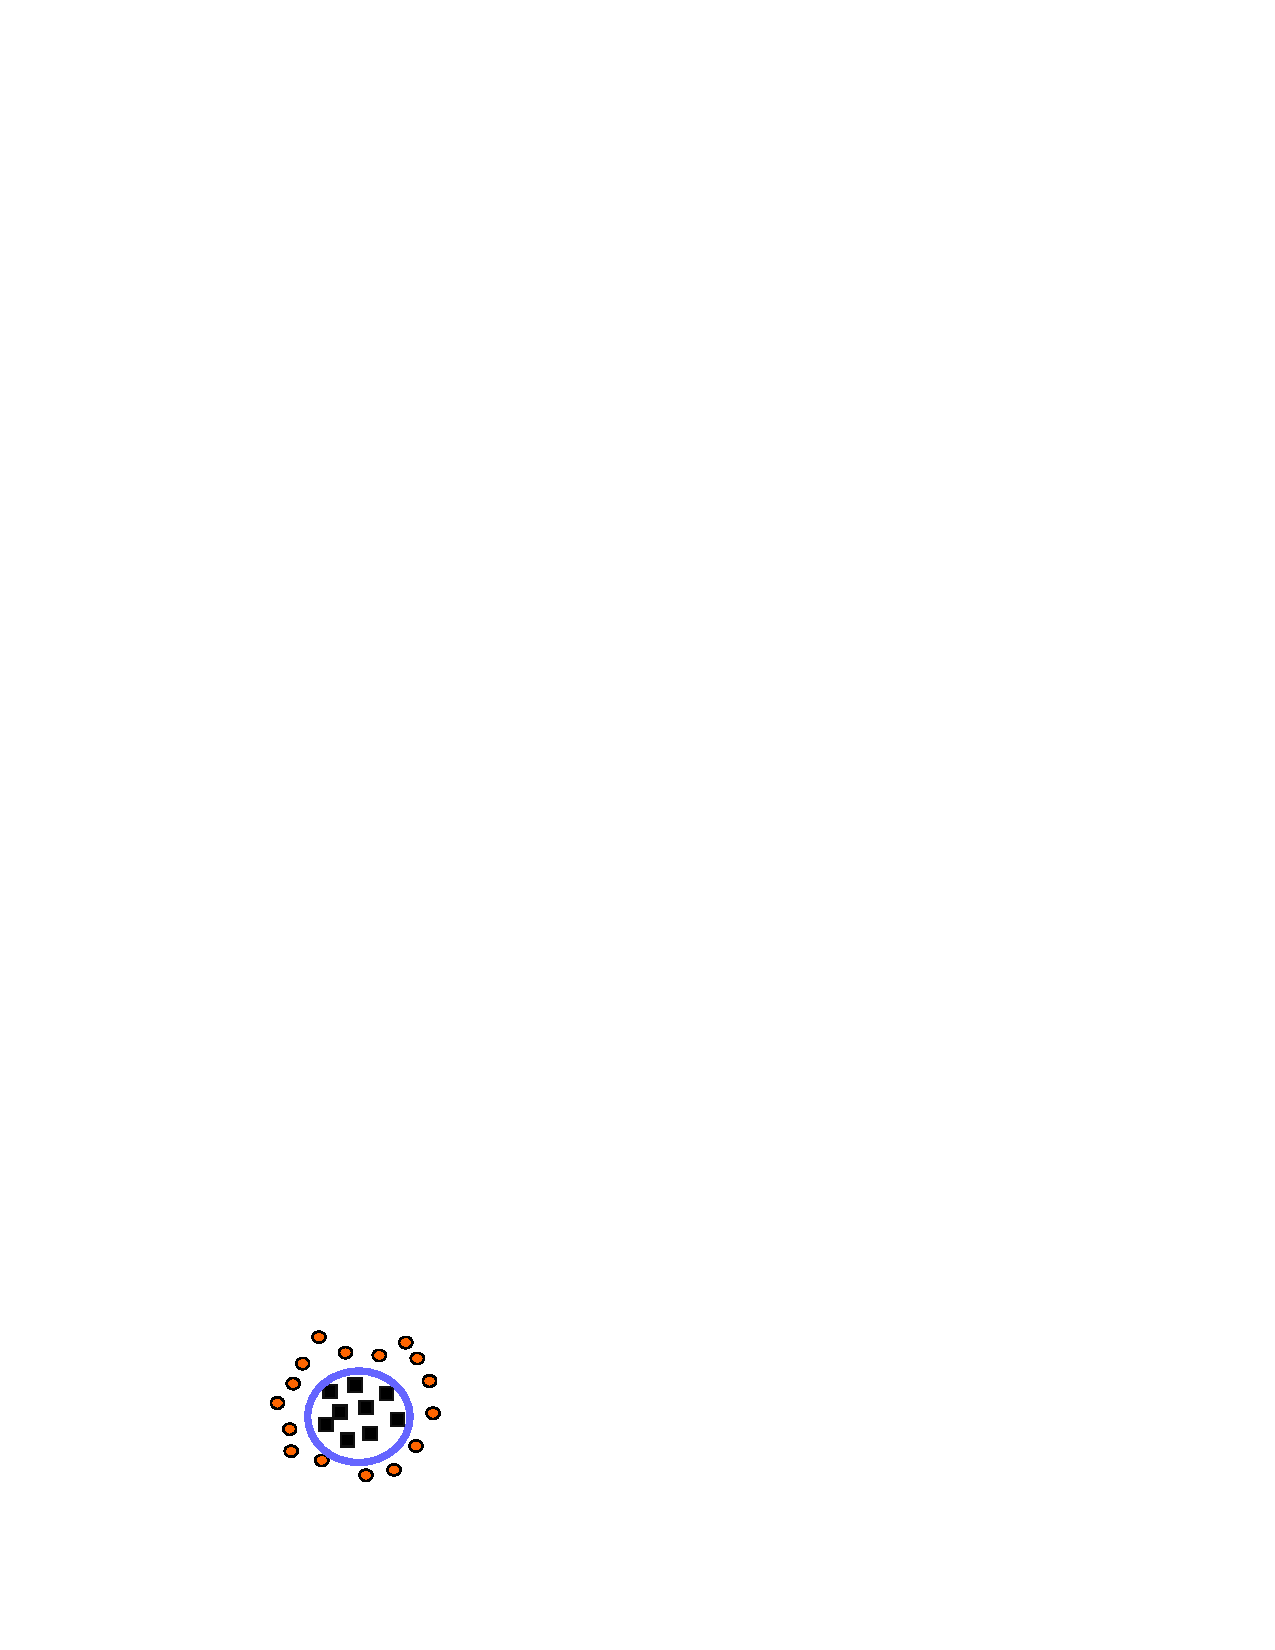
\includegraphics[width=0.66\textwidth]{svm_nl}
    \caption{Example of a non linear separation (quadratic discriminant)\cite{Bennett03supportvector}}
    \label{fig:svm_nonlin}
  \end{center}
\end{figure}

However, the speed of training and testing is low, even for fastest SVMs.
It is also directly limited to two-class tasks\cite{Cortes95support-vectornetworks},
requiring to reduce multi-class tasks to binary ones. Although, some work has been done to try to avoid
decomposing the problem in multiple binary class problems.\cite{Crammer:2002:AIM:944790.944813}

In the past few years, this method is also being used to classify internet traffic with excellent results.\cite{Yuan2010}


\subsubsection{KNN}

The \emph{k-nearest-neighbor} algorithm is among the most simple classification algorithms and it has been around since the 1950s \cite[p.348]{HanKam06}.
KNN is a non-parametric method which can be used in classification and regression problems and it is mostly used in the area of pattern recognition.
This algorithm is a type of instance-based learning, or lazy learning, which means that every computation is deferred until classification. By deferring 
computation to the classification phase this algorithm is slow at classifying instances. To classify a new instance, the algorithm has to calculate
the \emph{Euclidean distance} between the new instance and every instance in the training set.

Since the introduction of this algorithm, some variations of it appeared to help
solving the shortcomings of \emph{kNN}.\cite{DBLP:journals/corr/abs-1007-0085}
The more notable are:
\begin{itemize}
\item \textbf{Clustered k nearest neighbor} \cite{journals/jcp/ZhouLX09} is an improved version of k-nn mixed with a clustering algorithm, which allow, for example, 
better performance in classifying text.
\item \textbf{k-d tree nearest neighbor (kdNN)} \cite{Sproull1991} helps to improve, in some cases, the completion time of the classification in logarithmic time.
\item \textbf{Orthogonal Search Tree Nearest Neighbor} \cite{955110} greatly improves efficiency of k-nn, especially for large datasets.
\end{itemize}

\subsection{Clustering Algorithms}\label{sec:clust}

Clustering is the process of grouping similar entries/objects into different groups, in other words, it is the method of breaking a set into various subsets according to some
metric. This groups/subsets are not known from the start and clustering is sometimes considered the most important unsupervised learning problem\cite{DBLP:journals/corr/abs-1205-1117}.

Clustering methods can be divided into\cite{HanKam06}:
\begin{itemize}
\item \textbf{Partitioning Methods} start with an initial number of groups, and reallocates iteratively the elements on the groups
to convergence\cite{DBLP:journals/corr/abs-1205-1117}. Some examples of partitioning methods are based on heuristics like \emph{k-mean algorithm}
and \emph{k-medoids algorithm}.

\item \textbf{Hierarchical Methods} work by grouping data into a tree of clusters\cite{HanKam06}. This methods can be further divided into two
groups: \emph{agglomerative} (bottom-up) and \emph{divisive} (top-down)\cite{DBLP:journals/corr/abs-1205-1117}. At the beginning of an \emph{agglomerative} algorithm,
each object is a cluster and these clusters merge with each other, to form less but larger clusters. The opposite occurs for \emph{divisive} algorithms. The end 
condition for both is a distance threshold.\cite{HanKam06}

\item \textbf{Density-Based Methods} were developed to find clusters with odd forms, relying on the premise that the clusters are located in high density areas
that are separated from each other by low density zones \cite{HanKam06}. Some examples of algorithms which implement this method are \emph{DBSCAN} and \emph{SSN}.

\item \textbf{Grid-Based Methods} uses a multiresolution grid data structure. It divides the object space into a finite number of cells, that
form a grid structure, on which all of the operations for clustering are performed. This approach has a fast processing time,
which is typically independent from the number of data objects but, on other hand, dependent on the number of cells per dimension on the object space\cite{HanKam06}.
Some examples of algorithms which implement the rules of this method are \emph{STING},\emph{WaveCluster} and \emph{CLIQUE}.

\item \textbf{Model-Based Clustering Methods} tries to understand the mathematical rule behind the data, in other words, it is an
''attempt to optimize the fit between the given data and some mathematical model''\cite[p. 429]{HanKam06}. This method assumes 
that the data was generated with some underlying probability. Some examples of this algorithms are \emph{Expectation-Maximization},
\emph{Conceptual Clustering} and \emph{Neural Networks}.

\end{itemize}
%\subsection{Regression Algorithms}\label{sec:regr}
\subsection{Time Series Prediction}\label{sec:tsp}
One of the main problems, is to accurately predict the volumes of the inventory.
Since the data has temporal information one possible approach is to use time
series prediction to calculate future values of time series calculated from the
datasets.
\\

\cite{1716527} compared three forecasting techniques \emph{Support Vector
Machines} (SVMs), \emph{Multiple Regression} (MR) and \emph{Multilayer
Perceptron} (MLP), on power production values on multiple power plants. The
\emph{MR} outperformed the other two methods on predicting those values.
\\

\cite{Sabry:2007kq} compared \emph{ARIMA} with logistic regressions algorithms
to predict traffic on three Egyptian intercity roads. The average annual,
monthly and weekly daily traffic volumes were calculated using both logistic
regression and \emph{ARIMA} algorithms. They concluded that \emph{ARIMA} outperforms the
logistics regression methods in forecasting this traffic volumes.

\subsection{Data Mining Tools}
Today there are lots of free tools on the internet which can help us to test and use data mining techniques.
Some of the most used will be presented bellow.

\subsubsection{Weka}

Weka\footnote{ Available at \url{http://www.cs.waikato.ac.nz/~ml/weka/}} is a popular, open source, suite of machine learning software written in Java.
It was created at the University of Waikato, New Zealand in 1997. It has an easy to use and comprehensive GUI with access to an enormous deck of machine learning algorithms.

\begin{figure}[h]
  \begin{center}
    \leavevmode
    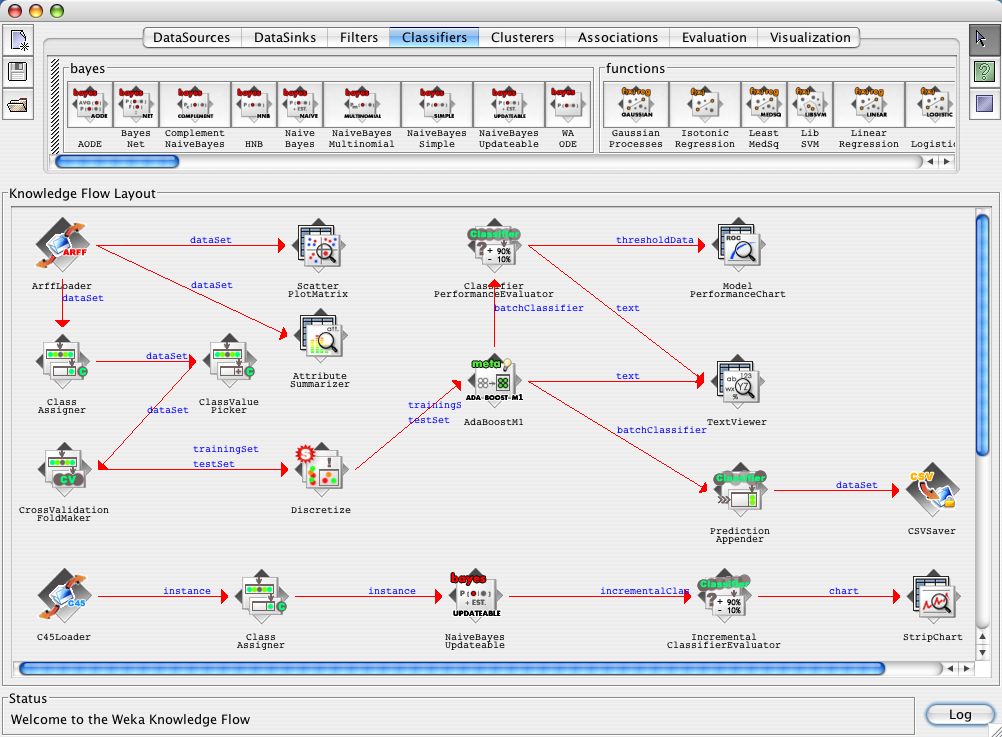
\includegraphics[width=0.66\textwidth]{wekaKF}
    \caption{Screenshot of Weka \protect\footnotemark}
    \label{fig:RapidMiner}
  \end{center}
\end{figure}
\footnotetext{ \url{http://www.siliconafrica.com/wp-content/themes/directorypress/thumbs//weka.png}}

\subsubsection{Apache Mahout}

Apache Mahout\footnote{ Available at \url{http://mahout.apache.org}} is an open source machine learning library to build scalable machine learning libraries.
Its core algorithms are implemented on top of map/reduce paradigm, to help in the scalability of the solution.
Since it is easier to get a cluster of server than an ultra high frequency CPU, and the market trend is to develop many and multi core solution, it is always the best option for processing large quantities of data scalable software.

According to their website, \emph{Mahout} has:
\begin{itemize}

\item User and Item based recommenders
\item Matrix factorization based recommenders
\item K-Means, Fuzzy K-Means clustering
\item Latent Dirichlet Allocation
\item Singular value decomposition
\item Logistic regression based classifier
\item Complementary Naive Bayes classifier
\item Random forest decision tree based classifier
\item High performance java collections (previously colt collections)
\item  A vibrant community

\end{itemize}

\subsubsection{RapidMiner}

Rapid Miner\footnote{ Available at \url{http://www.rapidminer.com/}} is a complete solution for data mining problems. It is available in a form of
a standalone GUI application.
\begin{figure}[h]
  \begin{center}
    \leavevmode
    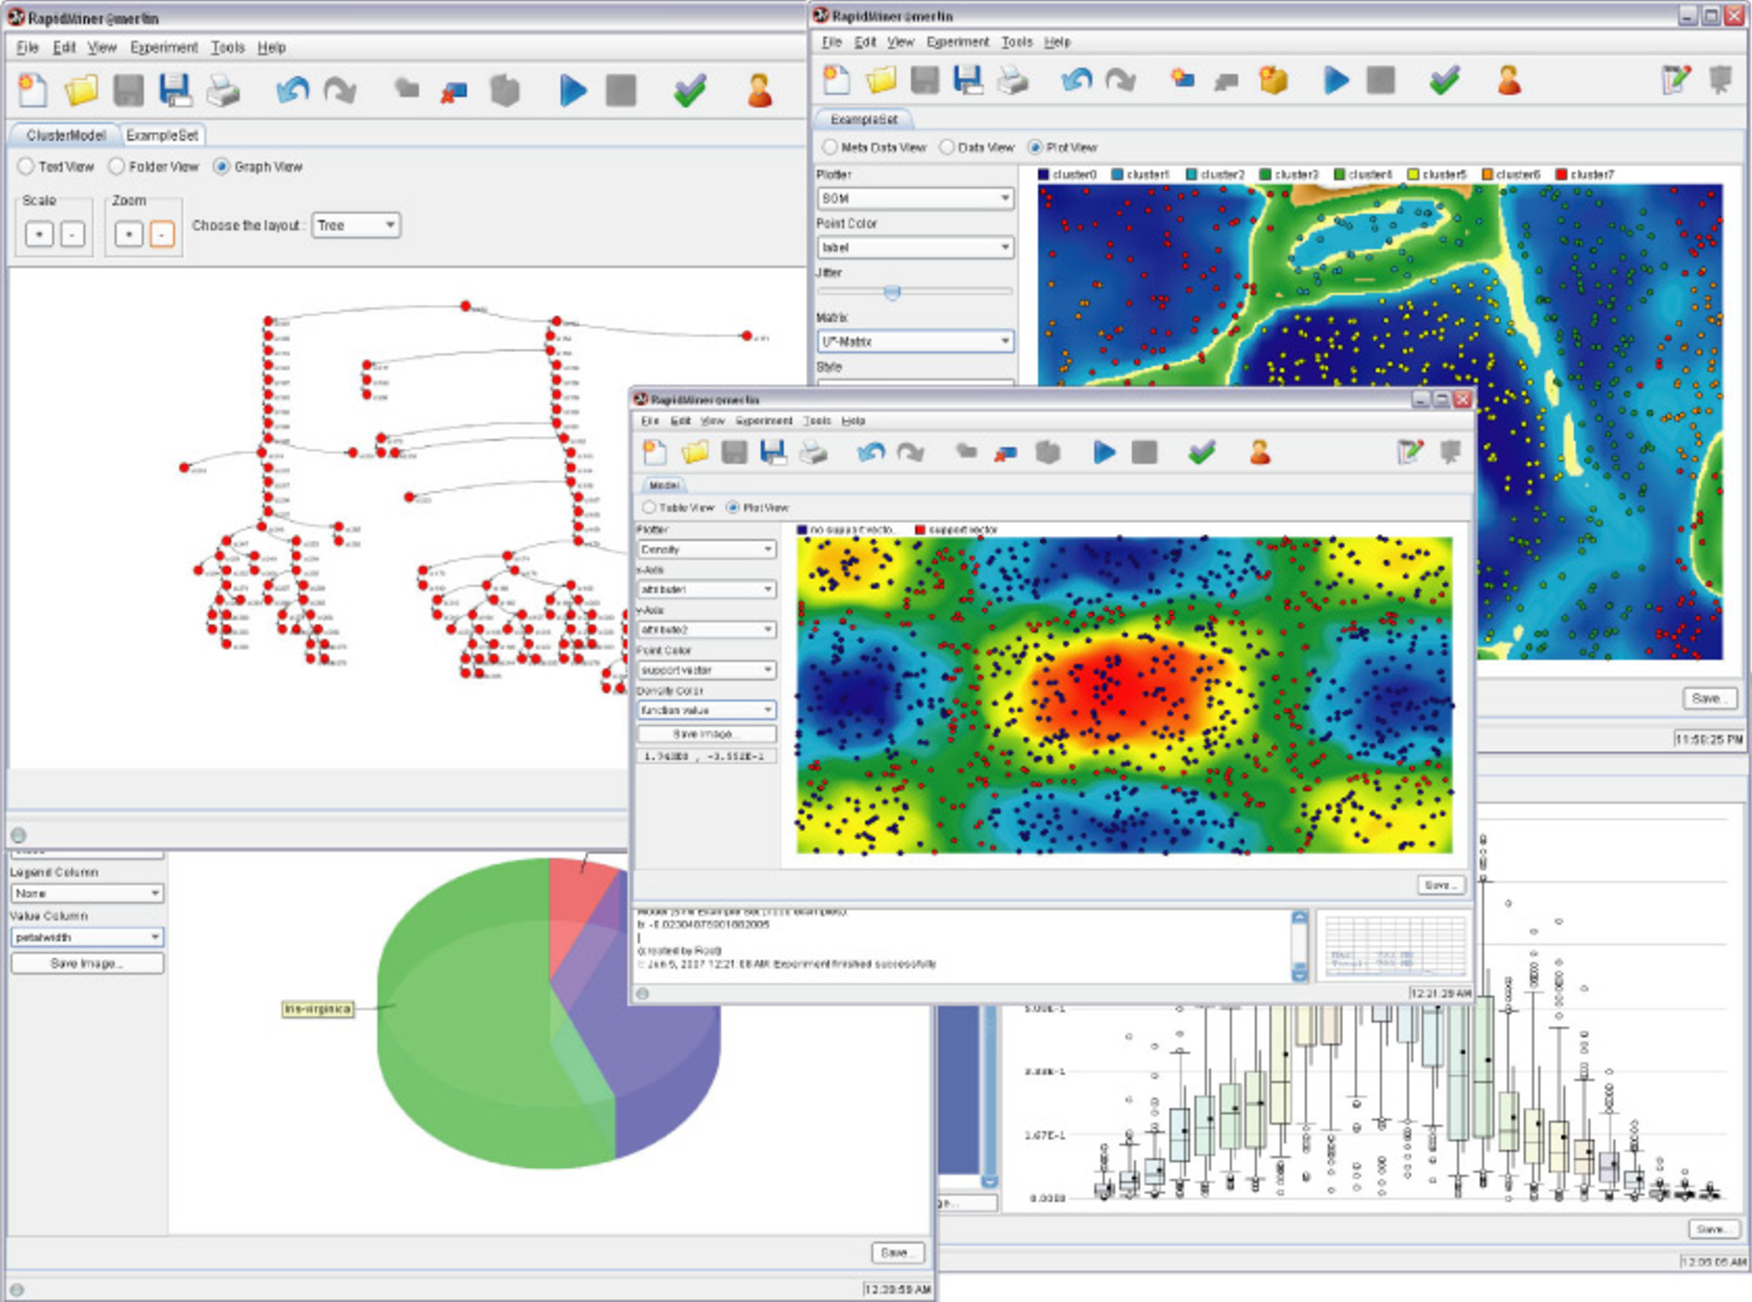
\includegraphics[width=0.66\textwidth]{rapidminer}
    \caption{Screenshot of RapidMiner \protect\footnotemark}
    \label{fig:RapidMiner}
  \end{center}
\end{figure}
\footnotetext{ \url{http://mloss.org/media/screenshot_archive/rapidminer_collection.jpg}}
 Although it is a commercial product, there is also a free tier, and the core and earliest versions are open source. This application
is one of the main players of this market and it is easily expandable through plug-ins available online.

\subsubsection{R Language}
R\footnote{ Available at \url{http://www.r-project.org}} is a free programming language and software environment for graphics generation and statistical computing.
Developed by Ross Ihaka and Robert Gentleman at the University of Auckland, New Zealand, in 1993 \cite{Ihaka98r:past}, it is still in active development and
greatly used by statistics and data miners.

R is an implementation of S, the statistics programming language, and it uses some characteristics inspired on Scheme.
R is a GNU tool, so it is completely free. There are wrappers to almost every language which can be used to access R variables from other programming languages.

\section{Model Evaluation Procedures and Measures}

To verify if a created model is valid it is necessary an additional step to validate the data.
This step can be divided into evaluation procedures, which normally
consists of dividing the original dataset into training and testing subsets, and
evaluation measures in order to assess the quality of our model.

\subsection{Model Evaluation Procedures}
\subsubsection{Cross-Validation}

This model consists of dividing the dataset in parts \cite{Witten:2005:DMP:1205860}
. Some of these parts will be used to train the model and other parts will only
be used in the validation part, so that we can assess if the model is able to
generalize the result or not. 

\paragraph{Sliding Window}

This procedure selects its training data and validation data maintaining the
chronological order of the data set\cite{Bensch_self-learningprediction}.

\begin{figure}[!h]
  \begin{center}
    \leavevmode
    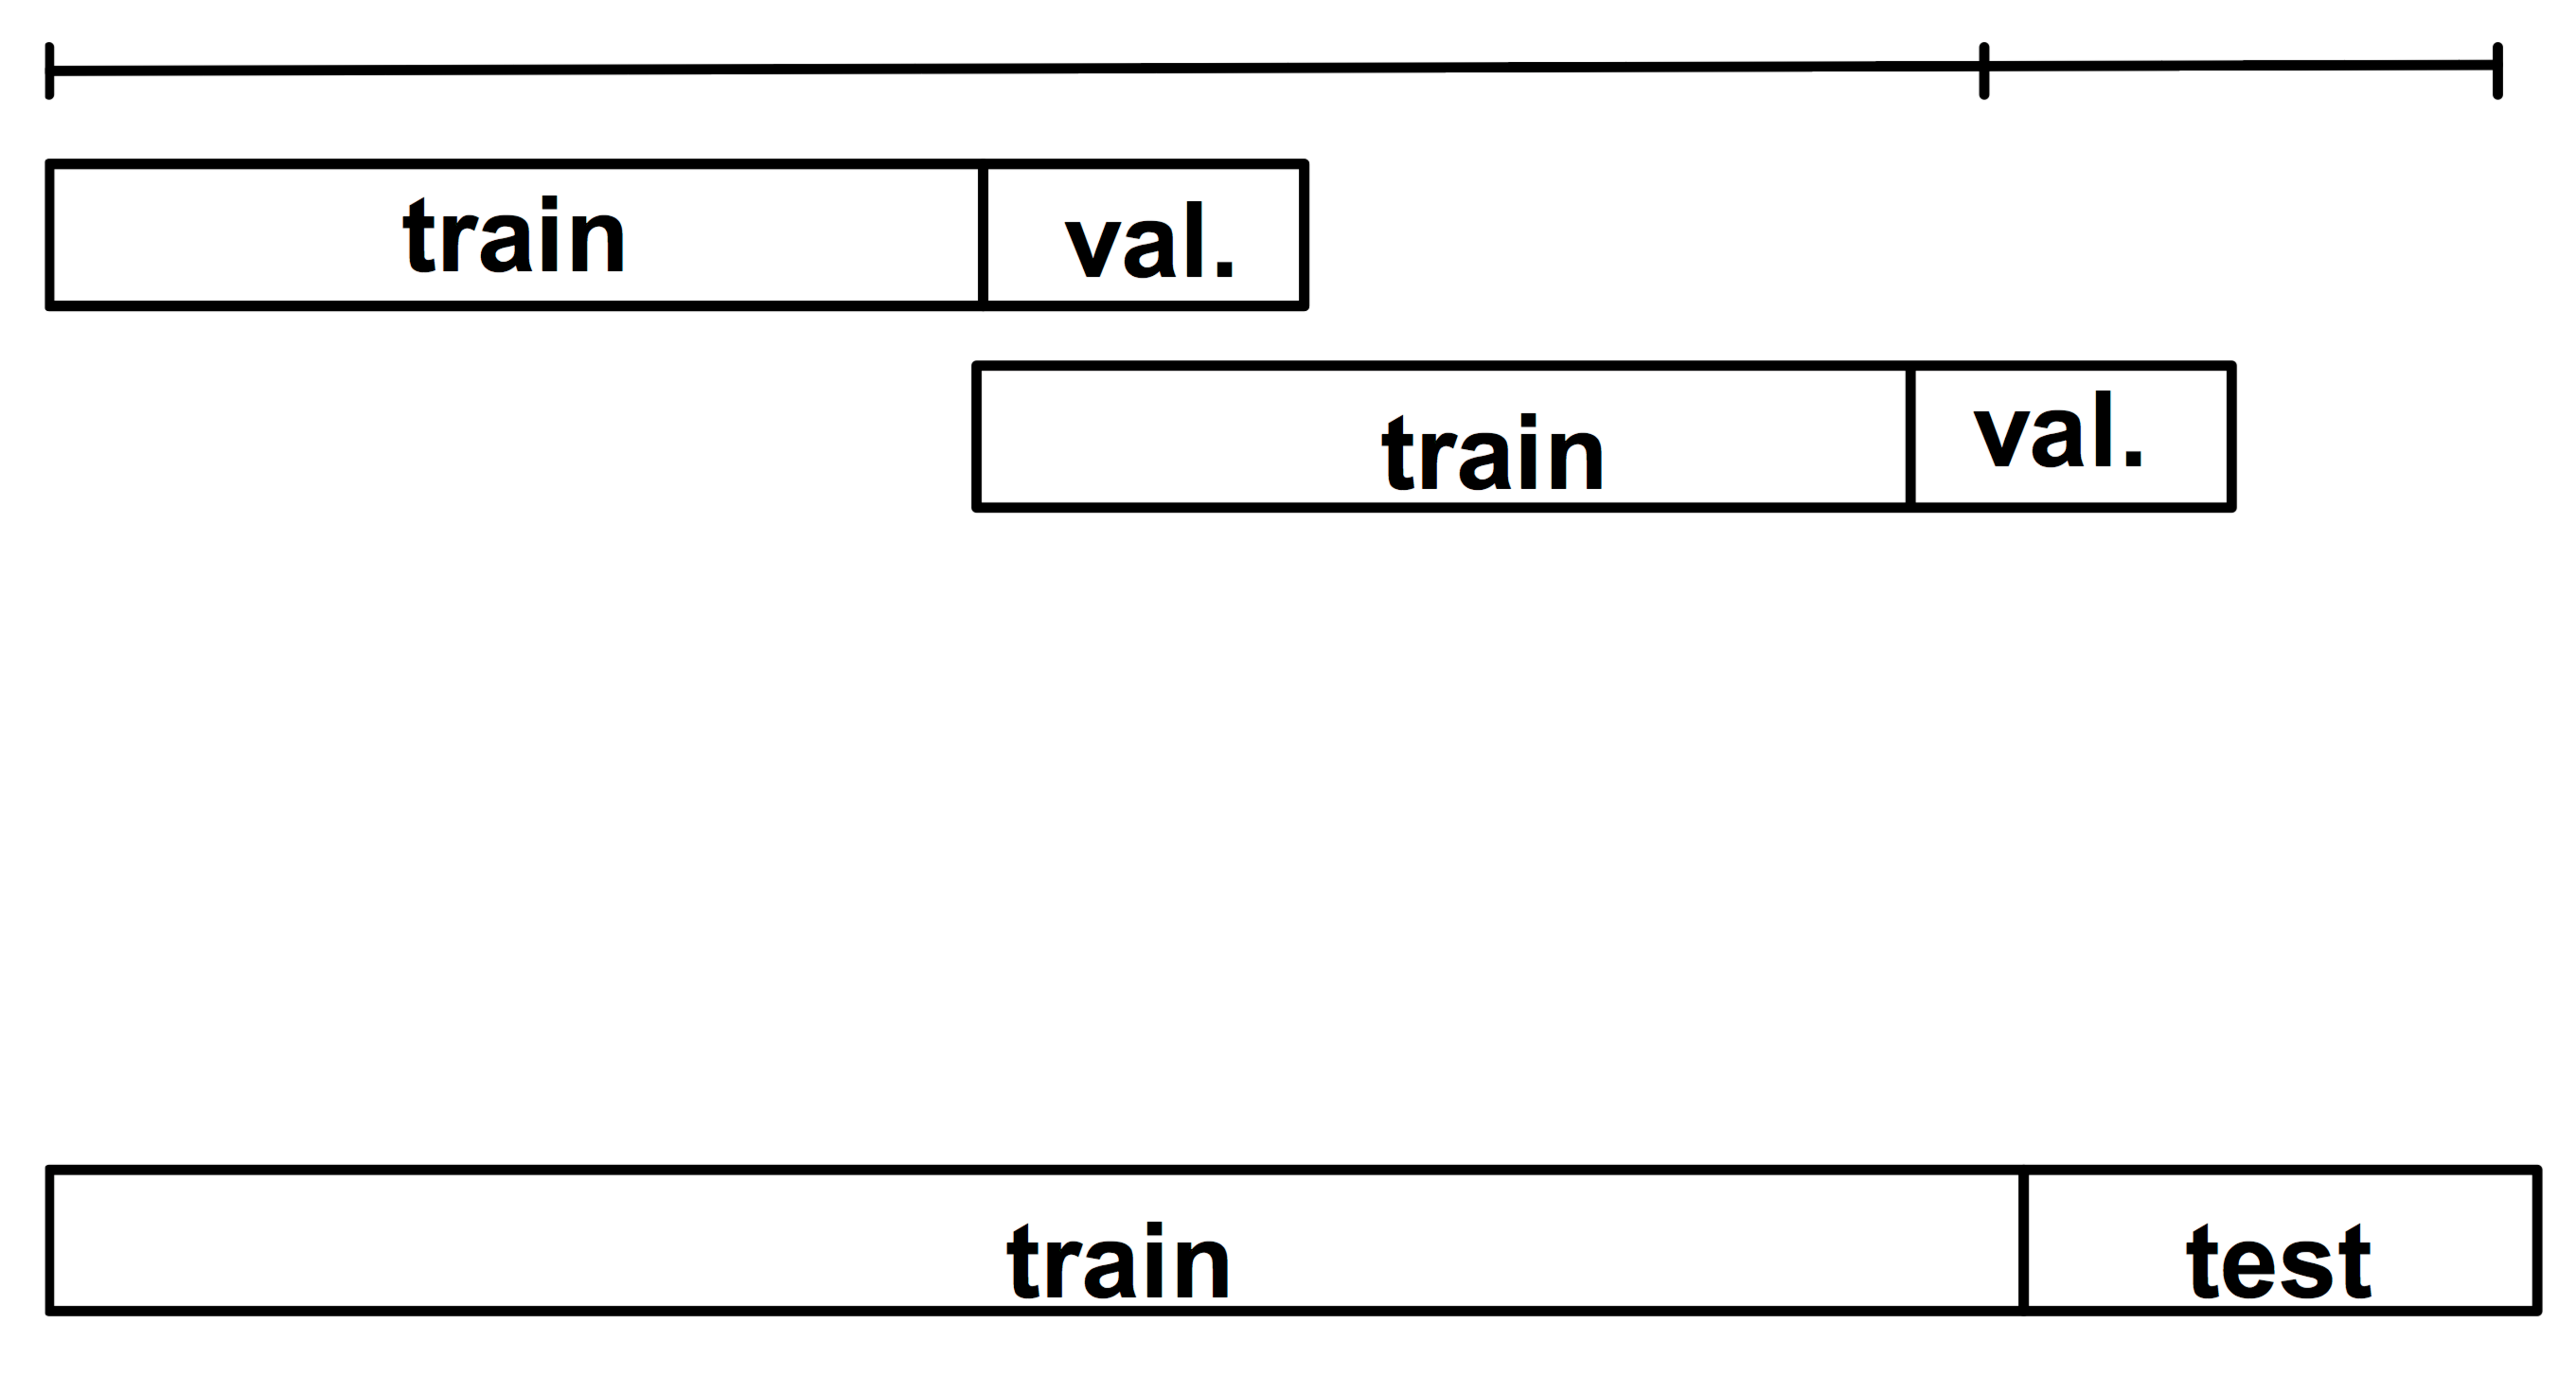
\includegraphics[width=0.66\textwidth]{swin}
    \caption{Sliding window validation}
    \label{fig:swin}
  \end{center}
\end{figure}
\FloatBarrier

In figure~\ref{fig:swin}, it possible to see that the validation data happens
after the training data in a temporal point of view.

\subsection{Model Evaluation Methods}

\subsubsection{Precision}

Precision is a metric to identify the fraction of positives that are correctly
classified as so. In other words, using this measure, we can identify how relevant the
results given by the algorithm are (the more higher the value, the more relevant
the results are). The equation to calculate precision is presented next:

\begin{center}
\Large
\begin{math}
Precision = \frac{\text{true positives}}{\text{true positives + false positives}}
\end{math}
\normalsize
\end{center}


\subsubsection{Recall}

This measure represents the part of actual positive results in the dataset that
were identified as such. In other words, recall is the fraction of positive
objects that were correctly identified by the algorithm from all the positive objects in the
dataset. This metric is calculated using the following expression:

\begin{center}
\Large
\begin{math}
Recall = \frac{\text{true positives}}{\text{true positives + false negatives}}
\end{math}
\normalsize
\end{center}

\subsubsection{Accuracy}

Accuracy represents the percentage of results that are actually correct. This
measure can be calculated as follows:

\begin{center}
\Large
\begin{math}
Accuracy = \frac{\text{true positives + true negatives}}{\text{true positives + false positives + true negatives + false negatives}}
\end{math}
\normalsize
\end{center}


\subsubsection{F-Measure}

F-Measure or F-Score or F\begin{math}_1 \end{math} measures the test accuracy relying in both recall
and precision. The best value of this function is 1 and the worst is 0.
F-Measure is the harmonic mean of the precision and recall and can be defined as
it follows:

\begin{center}
\Large
\begin{math}
F_1 = 2 * \frac{precision*recall}{precision+recall}
\end{math}
\normalsize
\end{center}

The reason behind the utilization of the harmonic mean instead of the arithmetic mean
is given due to a more intuitive result \cite{sasaki2007truth}.



\section{Web Usage Mining}\label{sec:network}

\nocite{UjwalaPatil}

The main area which this project focus on is the utilization of ad requests logs
to predict future requests of the users. This is analogous to work
which have been done in the area of user future requests prediction.
Next, it will be done a little overview of what has been studying in the area of web
usage data mining in the past years, in order to identify possible approaches
to solve the problem of this thesis.

\paragraph{}

In the area of pre-fetching web pages \cite{Nanopoulos01effectiveprediction}, it
has been proposed a new algorithm, WM\begin{math}_0\end{math}, which takes into
account the order between accesses and other specificities of the area. This
algorithm gets good results for accuracy even when compared to other methods
like \emph{Prediction-by-Partial-Match} (PPM) and \emph{Dependency Graph} (DG).

\paragraph{}

In another paper \cite{Gery:2003:EWU:956699.956716}, three approaches to
data mine from web logs are proposed. \textbf{Association Rule} (AR) is based on association rule
learning which is a very popular data mining family of algorithms to find relationships between
variables. The problem of finding web pages together in a web log is similar to
that problem. \textbf{Frequent Sequences} (FS), is a technique that tries to find time
ordered sequences of URLs that have been followed by past users.
\textbf{Frequent Generalized Sequences} (FGS) involves the utilization of a
generalized sequence, which is a
sequence that allows wild cards in order to represent a user flow of
navigation in a more flexible way. 
Some tests have been made by the author \cite{Gery:2003:EWU:956699.956716} to
test the performance of this three methods using real web logs. According to the
results given by FS, FS has better accuracy than AR and FGS.

\paragraph{}

In another paper, other author proposes a model that preserves sequentiality of
the clicks \cite{Frias-Martinez2003}. The rules maintain the sequence of the
click stream between the antecedent and the consequent, to maintain sequentiality.
This model also introduces the concept of temporality, which is reflected by the
distance between the consequent and antecedent by number of clicks to go from one
to the other. This rule is very important because it allows not only to find
which page is  going to be accessed but also when will it be accessed. The proposed
model, \textbf{Customizable Sequential Behavior Model}, can be adapted depending
on the characteristics of the server, in order to capture the behavior of the
users more accurately.

\paragraph{}

There is another approach that relies on the sequentially of the clicks
\cite{Jan:2007:WUB:1353862.1353874}.
This method uses the prefix set of web pages (pages that the user had already
visited) to predict a postfix set (next pages that the user will visit).
To select this pages, the algorithm uses a confidence threshold to select the pages
to the postfix set from historical data.


\paragraph{}

An approach based on the \textbf{Longest Common Subsequence} (LCS)
\cite{4631852} has also been used in web usage mining. In this case, the author
proposes a two part architecture: an offline part where knowledge is extracted
from the historical data and an online part where this knowledge is used to
predict the next visits of the user. The prediction is done in the online part by
appending the last request from the user to the history and using LCS. This
architecture is implemented in \textbf{WebPum} \cite{Jalali20106201} by the same
authors and improves the accuracy by a little margin from the
previous method, SUGGEST 3.0 \cite{1410804}, in the field of next page recommendations.

\paragraph{}

In other paper a method combining Markov model based sequential pattern
mining with clustering is proposed \cite{Anitha_anew}. This combination gets
about 12\% more accuracy when compared with the traditional Markov model.
The proposed models combine great accuracy from high order Markov Models with
less space complexity from low order Markov models.

\subsection{Web Usage Mining applied to Online Advertising}

Data mining is also being used to predict the response of an user to an online
ad\cite{chapelle2013simple}. Their main objective is to develop a framework that
can predict the result of an user clicking in an advertising, based on
the history that they have.
The proposed framework uses Maximum Entropy\cite{Nigam99usingmaximum}
because it is easy to implement, can be parallelized and scaled with respect
to the number of features. It is easy to include model updates in this method.
In this paper, they add a two-phase feature selection algorithm, to increase the
automation and reduce the need of domain expertise (a generalized mutual
information method to select the feature groups to be included and a feature
hashing to have the ability of controlling the size of the models). To their
experiments, the authors used logs with the same parameters as the datasets that
will be used on this project.

In another approach to the same problem are introduced improvements in the context of traditional
supervised learning based on FTRL-proximal online learning algorithm
\cite{McMahan:2013:ACP:2487575.2488200}. This paper also explores ways
to save memory during the prediction, using filters to select features to be
included in the model, such as \emph{Poisson Inclusion} and \emph{Bloom Filter
Inclusion}, and they concluded that the method which allows better savings,
without loosing much prediction accuracy, is \emph{Bloom Filter Inclusion}. To
solve the memory problem they also tested encoding values with fewer bits and
other techniques.

In yet another paper about CTR(Click-Through-Rate) prediction
\cite{Tagami:2013:CPC:2501040.2501978}, a two stage approach is used, the first
stage being the construction of a ranking model with the clicked ad requests and then a
sigmoid function converting the value of the ranking model into CTR. The method
proposed achieves better results in terms of AUC, MSE and LogLoss when compared
to: L2-loss linear SVM, logistic regression with only the clicked ad requests and
logistic regression with all the ad requests.

In the area of forecasting ad impressions, a Bayes network was used to capture
inter-dependencies between the query traffic features and the competitors in the
auction\cite{nath2013ad}. This method is used to forecast the number of
impressions of the ad to a certain keyword based on the bid that is done. Their
method, Generative Model based Ad Impression Forecasting Method, get better
results in terms of accuracy when compared to Normalized Bid Model. 
%\subsection{Instance-based regression algorithms}\label{sec:instance}
